% sizes tiny scriptsize footnotesize small normalsize large Large LARGE huge Huge

\documentclass[presentation]{beamer}

\usetheme{JuanLesPins}
\usecolortheme{orchid}
\setbeamertemplate{headline}{}
\setbeamertemplate{navigation symbols}{}

\usepackage{subfig}
\usepackage{graphicx}
\usepackage[english]{babel}
\usepackage[latin1]{inputenc}
\usepackage{color}
\usepackage{listings}
\definecolor{mygreen}{rgb}{0,0.6,0}
\definecolor{mygray}{rgb}{0.5,0.5,0.5}
\definecolor{mymauve}{rgb}{0.58,0,0.82}

\lstset{
  backgroundcolor=\color{white},   % choose the background color; you must add \usepackage{color} or \usepackage{xcolor}; should come as last argument
  basicstyle=\footnotesize\ttfamily, % the size of the fonts that are used for the code
  breakatwhitespace=false,         % sets if automatic breaks should only happen at whitespace
  breaklines=true,                 % sets automatic line breaking
  captionpos=b,                    % sets the caption-position to bottom
  commentstyle=\color{mygreen},    % comment style
  deletekeywords={...},            % if you want to delete keywords from the given language
  escapeinside={\%*}{*)},          % if you want to add LaTeX within your code
  extendedchars=true,              % lets you use non-ASCII characters; for 8-bits encodings only, does not work with UTF-8
  frame=single,	                   % adds a frame around the code
  keepspaces=true,                 % keeps spaces in text, useful for keeping indentation of code (possibly needs columns=flexible)
  keywordstyle=\color{blue},       % keyword style
  morekeywords={*,...},            % if you want to add more keywords to the set
  numbers=none,                    % where to put the line-numbers; possible values are (none, left, right)
  numbersep=5pt,                   % how far the line-numbers are from the code
  numberstyle=\tiny\color{mygray}, % the style that is used for the line-numbers
  rulecolor=\color{black},         % if not set, the frame-color may be changed on line-breaks within not-black text (e.g. comments (green here))
  showspaces=false,                % show spaces everywhere adding particular underscores; it overrides 'showstringspaces'
  showstringspaces=false,          % underline spaces within strings only
  showtabs=false,                  % show tabs within strings adding particular underscores
  stepnumber=2,                    % the step between two line-numbers. If it's 1, each line will be numbered
  stringstyle=\color{mymauve},     % string literal style
  tabsize=2,	                   % sets default tabsize to 2 spaces
  title=\lstname,                  % show the filename of files included with \lstinputlisting; also try caption instead of title
  linewidth=10.7cm,
}

\usepackage{tikz}


% Add any additional packages you use in your presentation
% -----pack
% \usepackage{xxx}
% -----
\usepackage{ragged2e}
\usepackage{tikz}
\usetikzlibrary{shadows}
\usetikzlibrary{positioning}

% Add your custom definitions etc., if required
% -----misc
% \newcommand{\xxx}[1]{[#1]}
% -----




\title{Reference counting}

\author[Miroslaw Blazej \&Miroslaw Blazej]
{%
   \texorpdfstring{
        \begin{columns}
            \column{.45\linewidth}
            \centering
            Miroslaw Blazej\\
            \href{mailto:blazej@student.agh.edu.pl}{blazej@student.agh.edu.pl}
            \column{.45\linewidth}
            \centering
            Michal Dygas\\
            \href{mailto:dygas@student.agh.edu.pl}{dygas@student.agh.edu.pl}
        \end{columns}
   }
   {Miroslaw \& Michal}
}
\institute[]{AGH University of Science and Technology}
\date{17-06-2020}


\begin{document}

\begin{frame}
  \titlepage
\end{frame}

\begin{frame}
  \frametitle{Introduction} 
  \justifying
 \textbf{Reference counting} is an \textbf{garbage collection} algorithm. It is based on \textbf{recording the number of pointers that points to given chunk of memory}. When the number of pointers drops to zero, the chunk can be declared garbage. 
 \\~\\
  In line with the name `reference counting`, in this presentation pointers will be called `references'.
  \\~\\
\end{frame}

\begin{frame}
  \frametitle{Basic rules (1)}
  \begin{columns}
    \begin{column}{0.5\textwidth}
      \begin{enumerate}
        \color{black} \item When a chunk is allocated from the heap, its reference count is initialized to \textbf{one}. 
        \color{gray} \item Whenever a reference to the chunk is \textbf{duplicated}, its reference count is \textbf{increased by one} (incremented).
        \color{gray} \item Whenever a reference to the chunk is \textbf{deleted}, its reference count is \textbf{decreased by one} (decremented).
        \color{gray} \item If the reference count \textbf{drops to 0}, the chunk \textbf{can be freed} because it is no longer reachable
      \end{enumerate}
    \end{column}
    \begin{column}{0.5\textwidth} 
      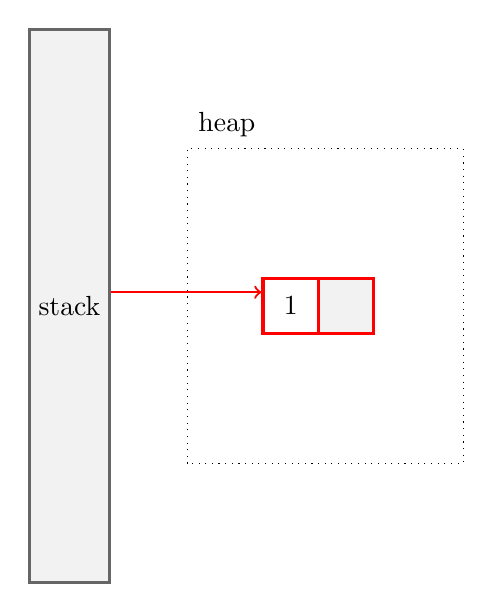
\begin{tikzpicture}[
        stack/.style={rectangle, draw=black!60, fill=black!5, very thick, minimum size=5mm, minimum height=200pt},
        count/.style={rectangle, draw=red, fill=white, very thick, minimum width=20pt, minimum height=20pt},
        chunk/.style={rectangle, draw=red, fill=black!5, very thick, minimum width=20pt, minimum height=20pt}
      ]
        \node[stack]  (stack)                                           {stack};
        \node[count]  (count)     [right of=stack, node distance=80pt]  {1};
        \node[chunk]  (chunk)     [right of=count, node distance=20pt]  {};

        \draw[red, ->, thick]     ([yshift=5pt]stack.east) -- ([yshift=5pt]count.west);

        \draw[black, dotted] (1.5, -2) rectangle (5, 2);
        \node[] at (2, 2.3) {heap};
      \end{tikzpicture}
    \end{column}
  \end{columns}
\end{frame}

\begin{frame}
  \frametitle{Basic rules (2)}
  \begin{columns}
    \begin{column}{0.5\textwidth}
      \begin{enumerate}
        \color{gray} \item When a chunk is allocated from the heap, its reference count is initialized to \textbf{one}. 
        \color{black} \item Whenever a reference to the chunk is \textbf{duplicated}, its reference count is \textbf{increased by one} (incremented).
        \color{gray} \item Whenever a reference to the chunk is \textbf{deleted}, its reference count is \textbf{decreased by one} (decremented).
        \color{gray} \item If the reference count \textbf{drops to 0}, the chunk \textbf{can be freed} because it is no longer reachable
      \end{enumerate}
    \end{column}
    \begin{column}{0.5\textwidth} 
      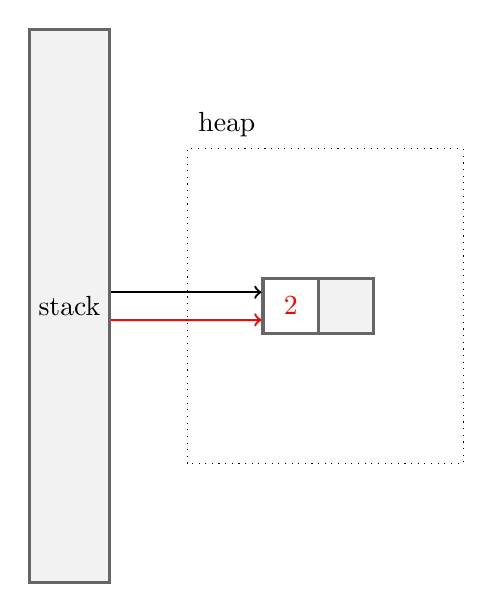
\begin{tikzpicture}[
        stack/.style={rectangle, draw=black!60, fill=black!5, very thick, minimum size=5mm, minimum height=200pt},
        count/.style={rectangle, draw=black!60, fill=white, very thick, minimum width=20pt, minimum height=20pt},
        chunk/.style={rectangle, draw=black!60, fill=black!5, very thick, minimum width=20pt, minimum height=20pt}
      ]
        \node[stack]  (stack)                                           {stack};
        \node[count]  (count)     [right of=stack, node distance=80pt, text=red]  {2};
        \node[chunk]  (chunk)     [right of=count, node distance=20pt]  {};

        \draw[->, thick]       ([yshift=5pt]stack.east) -- ([yshift=5pt]count.west);
        \draw[red, ->, thick]  ([yshift=-5pt]stack.east) -- ([yshift=-5pt]count.west);

        \draw[black, dotted] (1.5, -2) rectangle (5, 2);
        \node[] at (2, 2.3) {heap};
      \end{tikzpicture}
    \end{column}
  \end{columns}
\end{frame}

\begin{frame}
  \frametitle{Basic rules (3)}
  \begin{columns}
    \begin{column}{0.5\textwidth}
      \begin{enumerate}
        \color{gray} \item When a chunk is allocated from the heap, its reference count is initialized to \textbf{one}. 
        \color{gray} \item Whenever a reference to the chunk is \textbf{duplicated}, its reference count is \textbf{increased by one} (incremented).
        \color{black} \item Whenever a reference to the chunk is \textbf{deleted}, its reference count is \textbf{decreased by one} (decremented).
        \color{gray} \item If the reference count \textbf{drops to 0}, the chunk \textbf{can be freed} because it is no longer reachable
      \end{enumerate}
    \end{column}
    \begin{column}{0.5\textwidth} 
      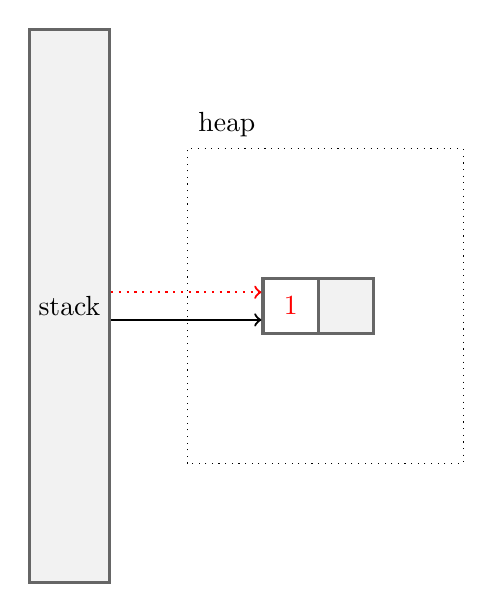
\begin{tikzpicture}[
        stack/.style={rectangle, draw=black!60, fill=black!5, very thick, minimum size=5mm, minimum height=200pt},
        count/.style={rectangle, draw=black!60, fill=white, very thick, minimum width=20pt, minimum height=20pt},
        chunk/.style={rectangle, draw=black!60, fill=black!5, very thick, minimum width=20pt, minimum height=20pt}
      ]
        \node[stack]  (stack)                                           {stack};
        \node[count]  (count)     [right of=stack, node distance=80pt, text=red]  {1};
        \node[chunk]  (chunk)     [right of=count, node distance=20pt]  {};

        \draw[red, ->, thick, dotted]       ([yshift=5pt]stack.east) -- ([yshift=5pt]count.west);
        \draw[->, thick]  ([yshift=-5pt]stack.east) -- ([yshift=-5pt]count.west);

        \draw[black, dotted] (1.5, -2) rectangle (5, 2);
        \node[] at (2, 2.3) {heap};
      \end{tikzpicture}
    \end{column}
  \end{columns}
\end{frame}

\begin{frame}
  \frametitle{Basic rules (4)}
  \begin{columns}
    \begin{column}{0.5\textwidth}
      \begin{enumerate}
        \color{gray} \item When a chunk is allocated from the heap, its reference count is initialized to \textbf{one}. 
        \color{gray} \item Whenever a reference to the chunk is \textbf{duplicated}, its reference count is \textbf{increased by one} (incremented).
        \color{gray} \item Whenever a reference to the chunk is \textbf{deleted}, its reference count is \textbf{decreased by one} (decremented).
        \color{black} \item If the reference count \textbf{drops to 0}, the chunk \textbf{can be freed} because it is no longer reachable
      \end{enumerate}
    \end{column}
    \begin{column}{0.5\textwidth} 
      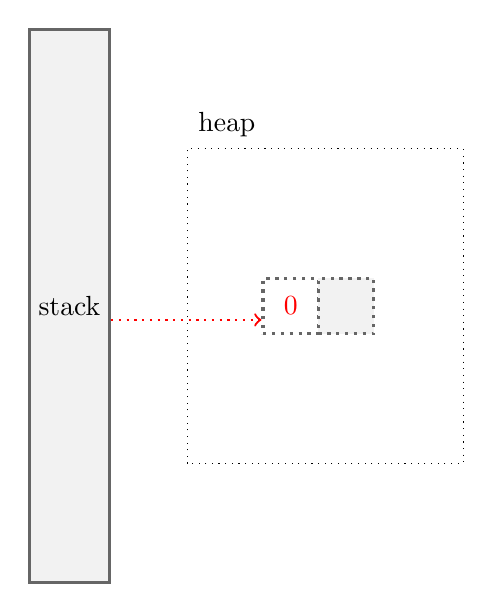
\begin{tikzpicture}[
        stack/.style={rectangle, draw=black!60, fill=black!5, very thick, minimum size=5mm, minimum height=200pt},
        count/.style={rectangle, draw=black!60, fill=white, very thick, minimum width=20pt, minimum height=20pt},
        chunk/.style={rectangle, draw=black!60, fill=black!5, very thick, minimum width=20pt, minimum height=20pt}
      ]
        \node[stack]  (stack)                                           {stack};
        \node[count, dotted]  (count)     [right of=stack, node distance=80pt, text=red]  {0};
        \node[chunk, dotted]  (chunk)     [right of=count, node distance=20pt]  {};

        \draw[red, ->, thick, dotted]  ([yshift=-5pt]stack.east) -- ([yshift=-5pt]count.west);

        \draw[black, dotted] (1.5, -2) rectangle (5, 2);
        \node[] at (2, 2.3) {heap};
      \end{tikzpicture}
    \end{column}
  \end{columns}
\end{frame}

\begin{frame}
  \frametitle{On-the-fly} 
  \justifying
Reference counting is \textbf{on-the-fly} type of garbage collector (also called incremental): some actions are performed at each call of \texttt{malloc} and/or \texttt{free}. These actions make some local modifications to the chunk structure to increase the probability of finding a free chunk
when needed.
\end{frame}


\begin{frame}
  \frametitle{Main implementation challenges}
  \justifying
    % \begin{block}{Implementation challenges}
        \begin{enumerate}
            \item keeping track of all
\textbf{reference manipulations}
            \item  recursively freeing chunks with zero reference count
        \end{enumerate}
    % \end{block}
\end{frame}

\begin{frame}
    \frametitle{Reference manipulations}
    \justifying
    The compiler \textbf{inserts special code for all reference manipulations} and at each call of \texttt{malloc} and/or \texttt{free} - incrementing
    the reference count when a reference to a chunk is duplicated and decrementing it
    when such a reference is deleted. 
      \\~\\
    Besides assignment statements, the compiler also has to add reference increasing code to \textbf{parameter transfers}, since
    a reference that is passed as a parameter is effectively assigned to a local variable of
    the called routine. Note that not all references in the running program are references to chunks on
    the heap; many of them point to blocks in the program data area, and all reference counting code must make sure it does not follow such references.

  \end{frame}


\begin{frame}
  \frametitle{p := q additional reference manipulations pseudocode}
  \justifying
  \begin{block}{}
  \textbf{if} Points into the heap (q):\\ \hspace*{20pt} Increment q.referenceCount;\\ \textbf{if} Points into the heap (p):\\ \hspace*{20pt} Decrement p.referenceCount;\\ \hspace*{20pt} \textbf{if} p.referenceCount = 0:\\ \hspace*{40pt} FreeRecursively (p);
  \end{block}
\end{frame}  

\begin{frame}
  \frametitle{recursively freeing chunks pseudocode}
  \justifying  
  \begin{block}{}
  \textbf{procedure} FreeRecursively(Pointer); \\
\hspace*{20pt} \textbf{if} not IsPointerIntoHeap (Pointer): \textbf{return};\\
\hspace*{20pt} \textbf{if} Pointer.referenceCount != 0: \textbf{return};\\
\hspace*{20pt} \textbf{for each} i \textbf{in} 1 .. Pointer.numberOfPointers: \\
\hspace*{40pt} \textbf{if} IsPointerIntoHeap (Pointer.pointer [i]): \\
\hspace*{60pt} Decrement Pointer.pointer [i].referenceCount; \\
\hspace*{60pt} FreeRecursively(Pointer.pointer [i]); \\
\hspace*{20pt} FreeChunk(Pointer); \\
  \end{block}
\end{frame}

\begin{frame}
  \frametitle{Recursively freeing cons} 
  \justifying
      \begin{alertblock}{Cons}
        Recursion is, however, an unwelcome feature in a garbage collector since it requires an \textbf{unpredictable amount of stack space}. 
\\~\\        
\justifying
        Having a garbage collector fail for lack of memory is kind of embarrassing, though, and several techniques
have been invented to avoid the problem. The best solution is using \textbf{pointer reversal}.
    \end{alertblock}
\end{frame}

\begin{frame}
  \frametitle{Identification techniques} 
  \justifying
  figures that will illustrate this algorithm
\end{frame}

\begin{frame}
  \frametitle{Identification techniques} 
  \justifying
  figures that will illustrate this algorithm
\end{frame}

\begin{frame}
  \frametitle{Algorithm issues} 
  \justifying
  \begin{alertblock}{Cons}
  	\begin{enumerate}
		\item efficiency
		\item memory fragmentation
		\item failes to reclaim a cyclic data structure 	
  	\end{enumerate}
  \end{alertblock}
\end{frame}


\begin{frame}
  \frametitle{Efficiency} 
  \justifying
The compiled code has
to monitor \textbf{all reference manipulations} and each and every reference manipulation
requires the adjustment of the associated reference counts. 
\\~\\
This is a considerable
\textbf{overhead} in comparison to other garbage collection techniques that do not monitor
any pointer action and reclaim garbage chunks only when needed.
\end{frame}

\begin{frame}
  \frametitle{Memory fragmentation} 
  \justifying
The free list is augmented with the reclaimed chunks, but it remains \textbf{fragmented}. In principle
doing a compaction phase during a reference counting allocation request is possible,
but few reference counting garbage collectors go to such lengths.

    \begin{figure}
        \centering
            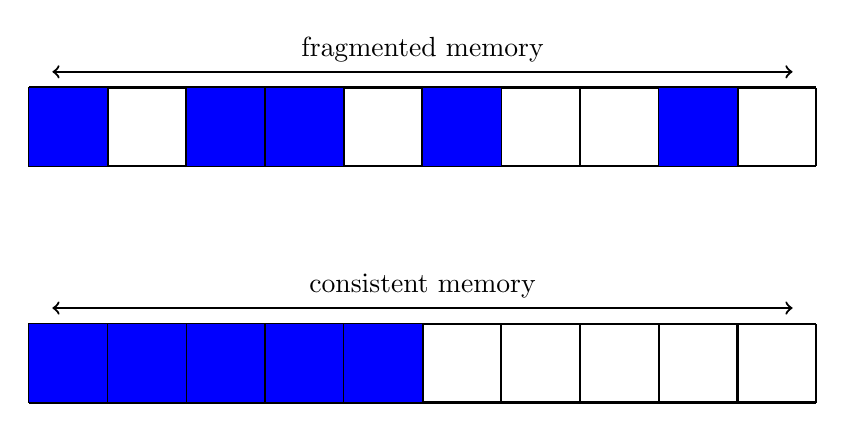
\begin{tikzpicture}
                \draw[thick, <->] (0.3, 1.2) -- (9.7, 1.2) node [midway, above, fill=white]{fragmented memory};
                
                \draw[thick] (0,0) grid (10,1);
                \filldraw[fill=blue, draw=black] (0,0) rectangle (1,1);
                \filldraw[fill=blue, draw=black] (2,0) rectangle (3,1);
                \filldraw[fill=blue, draw=black] (3,0) rectangle (4,1);
                \filldraw[fill=blue, draw=black] (5,0) rectangle (6,1);
                \filldraw[fill=blue, draw=black] (8,0) rectangle (9,1);
                   
				\draw[thick, <->] (0.3, -1.8) -- (9.7, -1.8) node [midway, above, fill=white] {consistent memory};
				                   
                \draw[thick] (0,-2) grid (10,-3);
                \filldraw[fill=blue, draw=black] (0,-2) rectangle (1,-3);
                \filldraw[fill=blue, draw=black] (1,-2) rectangle (2,-3);
                \filldraw[fill=blue, draw=black] (2,-2) rectangle (3,-3);
                \filldraw[fill=blue, draw=black] (3,-2) rectangle (4,-3);
                \filldraw[fill=blue, draw=black] (4,-2) rectangle (5,-3);
                
                
            \end{tikzpicture}
        \label{fig:compaction_example}
    \end{figure}

\end{frame}

\begin{frame}
  \frametitle{Cycles} 
  \justifying
The problem with reference counting is that it takes its decisions by considering
\textbf{only one node} in the graph at a time and \textsl{in order to reclaim a cyclic data structure all
nodes in the data structure should be considered as garbage together}. 
\\~\\
\justifying
Once reference counting has failed to reclaim a cyclic data structure, the chunks involved \textbf{will never
be reclaimed}. This has the unfortunate effect that free space leaks away, which might
even cause the program to run out of free space when other garbage collectors would
be able to reclaim the cyclic structures and allow the program to continue.
\\~\\

\end{frame}

\begin{frame}
  \frametitle{Cycles}
  \begin{columns}
    \begin{column}{0.5\textwidth}
      Despite deletion of last reference to chunk from stack, which causes that chunk is no longer available... 
      \\~\\
      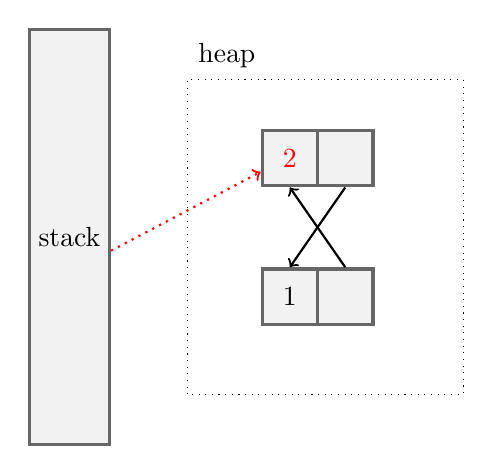
\begin{tikzpicture}[
        stack/.style={rectangle, draw=black!60, fill=black!5, very thick, minimum size=5mm, minimum height=150pt},
        count/.style={rectangle, draw=black!60, fill=black!5, very thick, minimum width=20pt, minimum height=20pt},
        chunk/.style={rectangle, draw=black!60, fill=black!5, very thick, minimum width=20pt, minimum height=20pt}
      ]
        \node[stack]  (stack)                                                                       {stack};
        \node[count]  (count)  at(2.8, 1)   [node distance=80pt, text=red]                  {2};
        \node[chunk]  (chunk)               [right of=count, node distance=20pt]            {};
        \node[count]  (count2) at(2.8, -1)  [below of=count, node distance=50pt]            {1};
        \node[chunk]  (chunk2)               [right of=count2, node distance=20pt]           {};

        \draw[red, ->, thick, dotted]  ([yshift=-5pt]stack.east) -- ([yshift=-5pt]count.west);
        \draw[->, thick]  (chunk.south) -- (count2.north);
        \draw[->, thick]  (chunk2.north) -- (count.south);

        \draw[black, dotted] (1.5, -2) rectangle (5, 2);
        \node[] at (2, 2.3) {heap};
      \end{tikzpicture}
    \end{column}
    \begin{column}{0.5\textwidth} 
      data is not deleted, as it is still referred by another chunk, kept alive by existing reference from our chunk
      \\~\\
      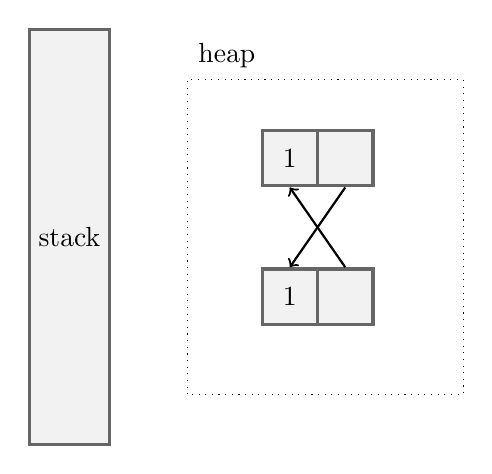
\begin{tikzpicture}[
        stack/.style={rectangle, draw=black!60, fill=black!5, very thick, minimum size=5mm, minimum height=150pt},
        count/.style={rectangle, draw=black!60, fill=black!5, very thick, minimum width=20pt, minimum height=20pt},
        chunk/.style={rectangle, draw=black!60, fill=black!5, very thick, minimum width=20pt, minimum height=20pt}
      ]
        \node[stack]  (stack)                                                                       {stack};
        \node[count]  (count)  at(2.8, 1)   [node distance=80pt]                            {1};
        \node[chunk]  (chunk)               [right of=count, node distance=20pt]            {};
        \node[count]  (count2) at(2.8, -1)  [below of=count, node distance=50pt]            {1};
        \node[chunk]  (chunk2)               [right of=count2, node distance=20pt]           {};

        \draw[->, thick]  (chunk.south) -- (count2.north);
        \draw[->, thick]  (chunk2.north) -- (count.south);

        \draw[black, dotted] (1.5, -2) rectangle (5, 2);
        \node[] at (2, 2.3) {heap};
      \end{tikzpicture}
    \end{column}
  \end{columns}
\end{frame}

\begin{frame}
  \frametitle{Weak references} 
  \justifying
  When using reference counting, cycles can be implemented using \textbf{weak references}. Creating, manupulating and deleting them does not cause changes of reference count.
  \\~\\
  However, chunk referenced by weak reference might no longer exist; programmer has to manually handle such situation.
  \\~\\
  \begin{columns}
    \begin{column}{0.4\textwidth}
      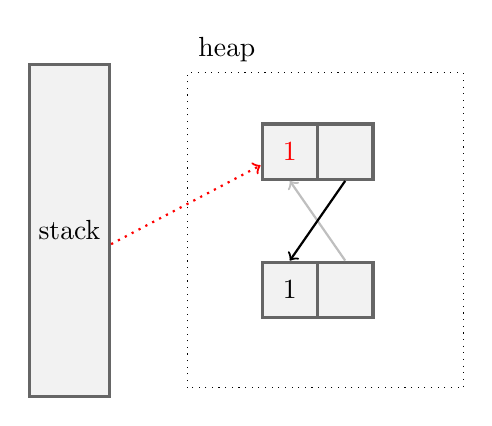
\begin{tikzpicture}[
        stack/.style={rectangle, draw=black!60, fill=black!5, very thick, minimum size=5mm, minimum height=120pt},
        count/.style={rectangle, draw=black!60, fill=black!5, very thick, minimum width=20pt, minimum height=20pt},
        chunk/.style={rectangle, draw=black!60, fill=black!5, very thick, minimum width=20pt, minimum height=20pt}
      ]
        \node[stack]  (stack)                                                                       {stack};
        \node[count]  (count)  at(2.8, 1)   [node distance=80pt, text=red]                  {1};
        \node[chunk]  (chunk)               [right of=count, node distance=20pt]            {};
        \node[count]  (count2) at(2.8, -1)  [below of=count, node distance=50pt]            {1};
        \node[chunk]  (chunk2)               [right of=count2, node distance=20pt]           {};

        \draw[->, thick, gray!50]  (chunk2.north) -- (count.south);
        \draw[red, ->, thick, dotted]  ([yshift=-5pt]stack.east) -- ([yshift=-5pt]count.west);
        \draw[->, thick]  (chunk.south) -- (count2.north);

        \draw[black, dotted] (1.5, -2) rectangle (5, 2);
        \node[] at (2, 2.3) {heap};
      \end{tikzpicture}
    \end{column}
    \begin{column}{0.1\textwidth} 
    \end{column}
    \begin{column}{0.5\textwidth} 
      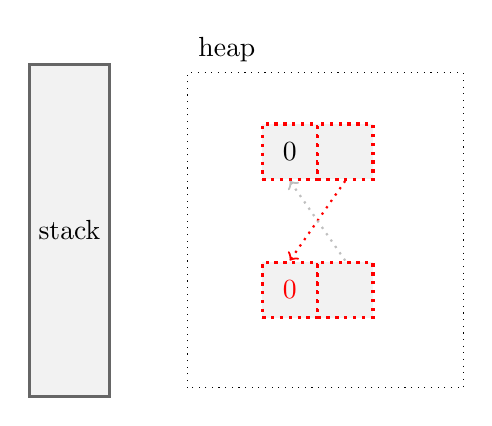
\begin{tikzpicture}[
        stack/.style={rectangle, draw=black!60, fill=black!5, very thick, minimum size=5mm, minimum height=120pt},
        count/.style={rectangle, dotted, draw=red, fill=black!5, very thick, minimum width=20pt, minimum height=20pt},
        chunk/.style={rectangle, dotted, draw=red, fill=black!5, very thick, minimum width=20pt, minimum height=20pt}
      ]
        \node[stack]  (stack)                                                                       {stack};
        \node[count]  (count)  at(2.8, 1)   [node distance=80pt]                            {0};
        \node[chunk]  (chunk)               [right of=count, node distance=20pt]            {};
        \node[count, text=red]  (count2) at(2.8, -1)  [below of=count, node distance=50pt]            {0};
        \node[chunk]  (chunk2)               [right of=count2, node distance=20pt]           {};

        \draw[->, thick, dotted, red]  (chunk.south) -- (count2.north);
        \draw[->, thick, dotted, gray!50]  (chunk2.north) -- (count.south);

        \draw[black, dotted] (1.5, -2) rectangle (5, 2);
        \node[] at (2, 2.3) {heap};
      \end{tikzpicture}
    \end{column}
  \end{columns}
\end{frame}

\begin{frame}
  \frametitle{Reference counting in parallel programming} 
  \justifying
  Reference counting is based on modyfing (incrementing or decrementing) a value every time reference is copied/dropped. If reference is shared between threads, more than one thread might try to copy/drop reference, causing \textbf{data race}.
  \\~\\
  This problem can be solved by making reference count an \textbf{atomic} variable. It solves problems with data races, hovewer - as atomic operations are expensive - it decerases performance. 
\end{frame}

\begin{frame}[fragile]
  \frametitle{Usage of reference counting - Objective-C, Swift} 
  \justifying
  Reference counting is used as method of garbage collection in languages related to Apple ecosystem - \textbf{Objective-C} and \textbf{Swift}.
  \\~\\
  In order to allow cyclic data structures, Objective-C and Swift allows creating weak references using \texttt{weak} keyowrd:
  \\~\\
  \begin{lstlisting}
    class Person {
      var apartment: Apartment
    }

    class Apartment {
      weak var tenant: Person?
    }\end{lstlisting}
\end{frame}

\begin{frame}[fragile]
  \frametitle{Usage of reference counting - smart pointers} 
  \justifying
  Reference counting is also often used in \textbf{smart pointers}. Smart pointers are data structures that wraps raw pointers and manages data that it points to, providing garbage collection. They are \textbf{not a part of language itself} - they are usually part of standard library. 
  \\~\\
  For example, C++ standard library provides \texttt{shared\_ptr} and \texttt{weak\_ptr} template classes, which implements reference counting:
  \\~\\
  \begin{lstlisting}[
    basicstyle=\tiny
  ]
    shared_ptr<Person> person1 = make_shared<Person>(Person()) // refcount = 1
    shared_ptr<Person> person2 = person // refcount = 2
    weak_ptr<Person> person_weak = weak_ptr<Person>(person1) // refcount = 2\end{lstlisting}
  % \\~\\
  C++ mechanisms such as copying constructors, operator overloading and RAII allows smart pointers to use natural C++ idioms without need of directly implementing GC in the compiler.
\end{frame}

\begin{frame}[fragile]
  \frametitle{Usage of reference counting - other} 
  \justifying
  \textbf{Rust} also provides smart pointers types in its standard library. As avoiding data races in compile-time is main goal of Rust, Rust standard library provides 3 types of smart pointers: 
  \begin{itemize}
    \item \texttt{Rc<T>} - does not use atomic variable for counting reference, cannot be sent to other threads (enforced in compile-time)
    \item \texttt{Arc<T>} - uses atomic variable for counting reference, can be sent to other threads
    \item \texttt{Weak<T>} - weak reference
  \end{itemize}
  \vspace{20pt}
  Reference counting is also usually used in \textbf{UNIX} kernels for handling \textbf{file descriptiors recovery}.
\end{frame}


\end{document}
